\documentclass[12pt,pdftex,preprint]{aastex}

\newcommand{\documentname}{\textsl{Article}}
\newcommand{\etal}{\textit{et~al.}}
\newcommand{\project}[1]{\textsl{#1}}
\newcommand{\test}{\mathrm{test}}

\begin{document}

\title{DRAFT: A precise data-driven model for high-dynamic-range imaging}

\author{Rob~Fergus\altaffilmark{1, 2},
        David~W.~Hogg\altaffilmark{3},
        Ben~R.~Oppenheimer\altaffilmark{4},
        Douglas~Brenner\altaffilmark{4},
        others}
\altaffiltext{1}{Department of Computer Science, New York University}
\altaffiltext{2}{to whom correspondence should be addressed: fergus@cs.nyu.edu}
\altaffiltext{3}{Center for Cosmology and Particle Physics, Department of Physics, New York University, 4 Washington Pl, New York, NY 10003}
\altaffiltext{4}{Department of Astrophysics, American Museum of Natural History}

\begin{abstract}
High dynamic-range imagers aim to block out or null light from a very
bright primary star to make it possible to detect and measure far
fainter companions; in real systems a small fraction of the primary
light is scattered, diffracted, and unocculted.  We build a flexible
data-driven model for the unocculted (and highly speckled) light in
the \project{P1640} spectroscopic coronograph to make very sensitive
detections and measurements.  The model is designed to be able to
capture the spatial structure and wavelength dependence of the
speckles but not the signal produced by any companion.  The model
includes a PCA that can capture the irregular expansion of the speckle
pattern with wavelength, which for each proposed companion position is
trained on pixels not overlapping the proposed position.  We find that
we are sensitive to companions that are of order a percent of the
brightness of the speckles, or hundreds (?) of thousands of times
fainter than the primary star in the data we have, outperforming
existing methods by a factor of ten.
\end{abstract}

\section{Introduction}

High dynamic range imaging and spectroscopy is the next frontier in
the study of exoplanets.  There is hope for atmospheric spectroscopy
of substantial numbers of giant planets, direct detection of planets
at large albedo and radius, and eventually---with something like the
far-future \project{Terrestrial Planet Finder}---direct time-domain
imaging and spectroscopy of Earth-like planets around other stars.
All of these projects involve exceedingly precise optical designs, in
which the light from the (generally bright) primary star is
more-or-less nulled, at least for certain locations on the focal
plane.  Perfect nulling is almost never possible, because it requires
sub-wavelength control of extremely large optical surfaces and the
wavefronts reflected from them.  There is no future of these projects
without very sophisticated instrument models and software pipelines
that implement them.

A working example is the \project{P1640} spectroscopic coronograph
(\citealt{p1640}).  It [has the following characteristics and
  successes].  The images produced by \project{P1640} have the vast
majority of the light from the primary star nulled at the focal plane.
The remaining light falls in a highly speckled pattern produced by
constructive and destructive interference of residual imperfections in
the wavefronts entering the instrument, made worse by differential
chromatic aberration.  The speckle pattern is quasi-random but has
some overall variation with wavelength, somewhat like the pure angular
expansion with wavelength that would be expected for perfect optics,
but not exactly. [Show some example data here; demonstrate
  regularities \emph{and} variation].

In principle, a wavelength-level model of the wavefronts and all
optical (and non-optical) surfaces in the \project{P1640} system would
produce a precise model of the intensity maps read out at the
detector.  Naively, this model would have of order $10^{12}$
parameters and be intractable to instantiate, let alone fit or
optimize.  Without this model, the speckles are stochastic but with
strong regularities.  This suggests data-driven modeling, or using the
\emph{data that the instrument has in fact taken} to build a precise
and informative but flexible model of the data that it \emph{can}
produce.  If this model can be trained on data that don't have---or
aren't expected to have---faint companions contributing, then
companions can be detected as failures of the model, or successes of a
model that is a superposition of the data-driven model and a model
companion.

Of course, we don't know in advance what stars will have companions,
and what won't; we don't have tagged data for training what are known
as ``supervised'' methods.  Relying on the fact that companions are
extremely rare, we adopt a ``train and test'' framework, in which we
use, when looking for a companion at a particular location in the
focal plane, all the data in the data set \emph{not} at that location
to train the model.  At the same time, we have very severe precision
requirements, because we are looking for companions that are far
fainter than the residual intensity in the instrument.  This latter
requirement pushes us towards models for the unblocked light that are
extremely flexible, but not so flexible that they can absorb light
from companions.  We will end up getting good performance by using
models with dozens to hundreds of parameters in every small patch of
the focal plane.

In this \documentname, we present a new methodology for modeling high
dynamic-range data that is extremely effective when the images are
spectroscopically sliced.  We demonstrate the method with
\project{P1640} data, and release working code.

\section{Method}

[perhaps here a bit of an overview of how the instrument works]

From the perspective of this \documentname, the \project{P1640}
instrument produces properly calibrated intensity information $I_{x y
  \lambda n}$ on a four-dimensional boxel grid where the $(x, y)$
indices indicate a pixel number on a regular square pixel grid in the
focal plane, the $\lambda$ index indicates one of a set of narrow
wavelength bins, and the $n$ index is exposure index or epoch number
in the multiple exposures that make up the data set for any one star.
The \project{P1640} instrument does not directly deliver data in this
form; it has to be processed into this form by a non-trivial
calibration and rectification pipeline (reference) that is outside our
current scope.  In brief, we are going to build a model for small
patches of this data by taking representative sets of patches
(training sets) and building a PCA-based data-driven model for
patches.

We locate the optical center of the system in the image (the location
of the star, which---ideally---is centered on the coronographic stop.
This involves centroiding four control spots created by reflections of
a tiny fraction of the primary light in the instrument.  Relative to
this located center, we transform the data from cartesian $I_{x y
  \lambda n}$ to polar $D_{r \theta \lambda n}$ coordinates, where
again the subscripts are indices but now $r$ indicates radial bin, and
$\theta$ indicates angular bin in the polar grid.  There are $R\sim
100$ radial bins ($1\leq r\leq R$), $\Theta\sim 300$ angular bins
($1\leq\theta\leq\Theta$), $\Lambda\sim 30$ wavelength bins
($1\leq\theta\leq\Theta$), and $N\sim 10$ exposures ($1\leq
n\leq N$) for typical exposure sequences.  That is, the full data
object $D_{r \theta \lambda n}$ has size (number of voxels)
$[R\times\Theta\times\Lambda\times N]$.  We use symbol $D$ for the
transformed data and not $I$ because in the transformation we
multiplied by a ratio of volumes to flatten a bit the dynamic range
[Fergus, is this correct, and do you also whiten the data?].


\begin{figure}[h!]
\begin{center}
\mbox{
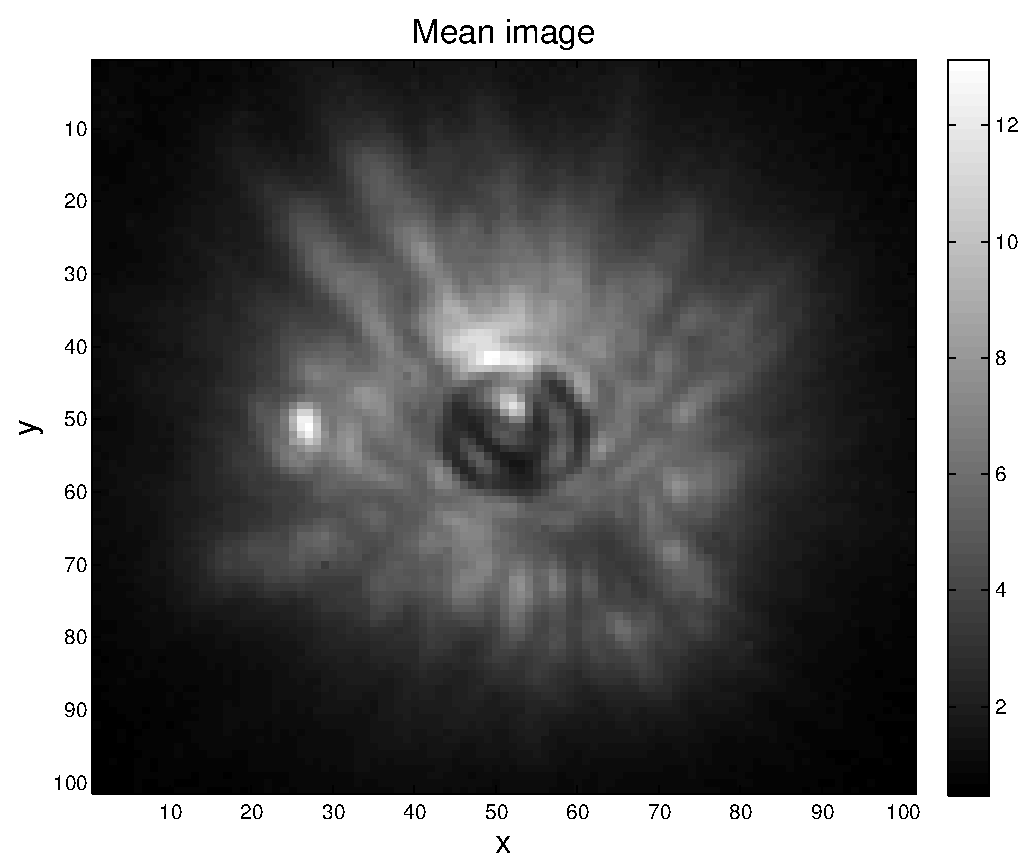
\includegraphics[width=2.5in]{figs/mean_xy.pdf}
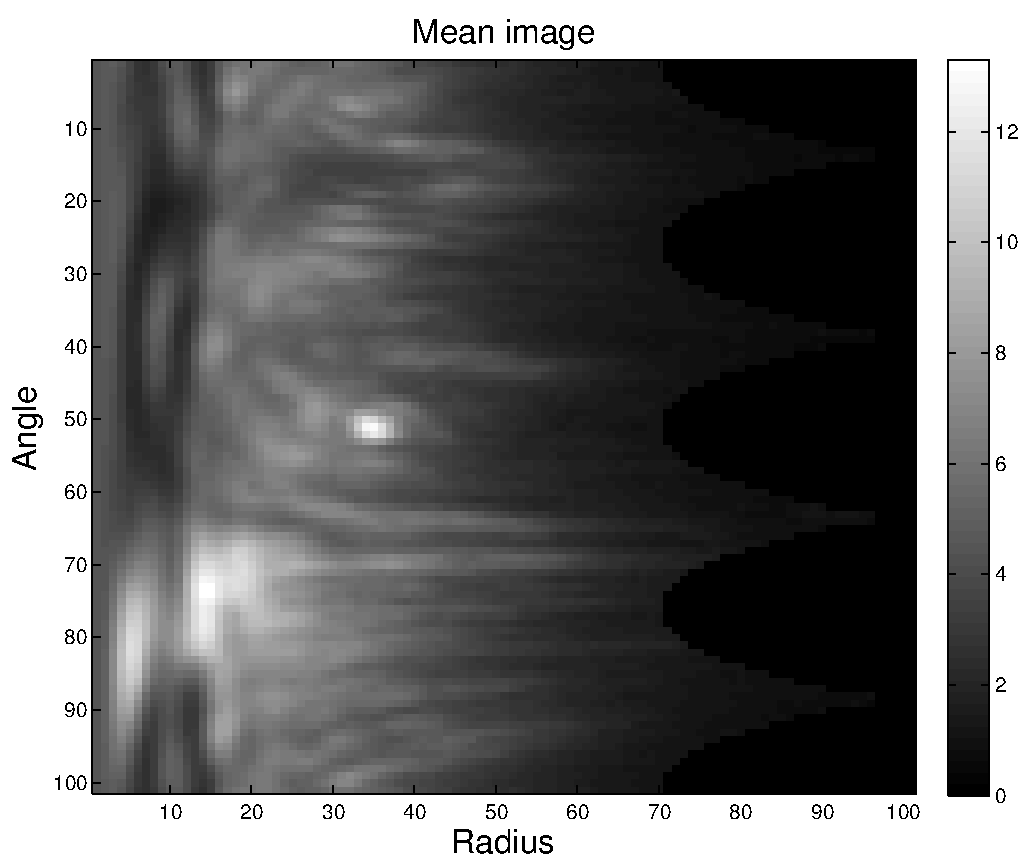
\includegraphics[width=2.5in]{figs/mean_rt.pdf}
}
\end{center}
\vspace{-7mm}
\caption{Mean over wavelength and cubes for the star
 FU ORI. Left:
  Cartesian representation. Right: Polar representation.}
\label{fig:mean}
\end{figure}
 

The data is modeled in tiny \emph{patches} $P_{r \theta n}$, which are
cutouts of size $[W\times 3\times\Lambda\times 1]$ from the full data
object.  These have a width $W\sim 31$~pix in the radial direction,
3~pix in the angular direction, but cover the full wavelength range
from a single exposure.  Each patches consists of a few thousand
contiguous data voxels.  In the most trivial radially symmetric model
for the instrument, the wavelength dependence of the data should be
purely linear radial expansion with wavelength.  The ``shape'' of the
patches permits the model to capture this behavior easily by
containing a significant radial domain and the full wavelength domain.
The 3~pix angular domain permits the model to find angular correlates
of departures from the purely radial expectation.  We chose the
angular width of 3~pix by trial and error; large values increase the
expense of the PCA (below) without much performance benefit.


\begin{figure}[h!]
\begin{center}
\mbox{
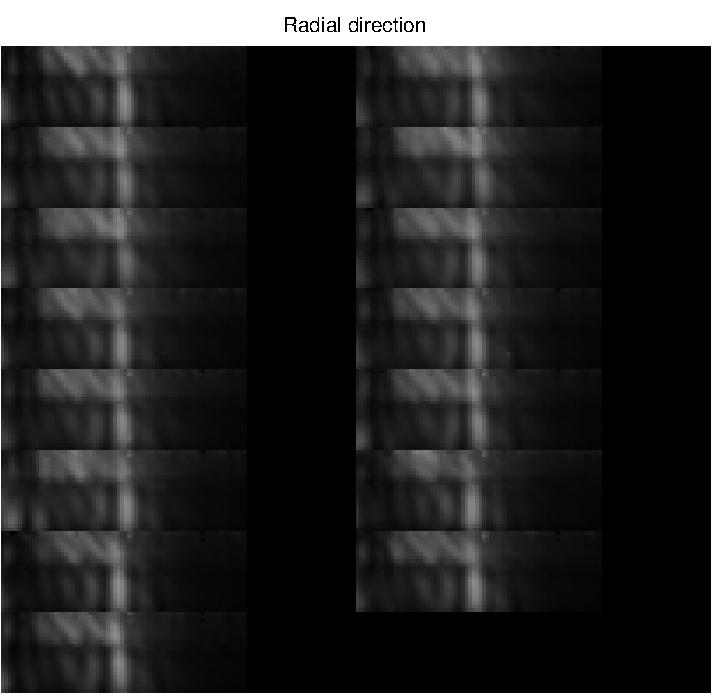
\includegraphics[width=2.5in]{figs/radius.pdf}
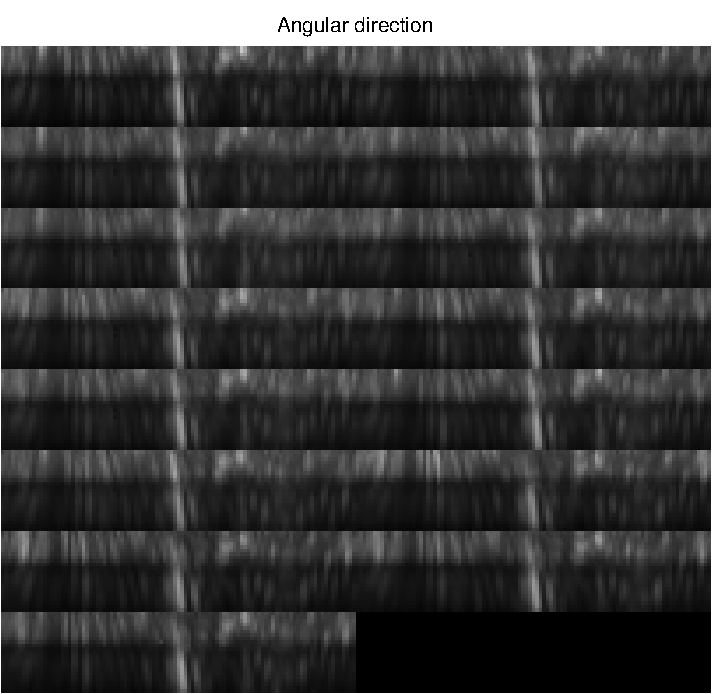
\includegraphics[width=2.5in]{figs/theta.pdf}
}
\end{center}
\vspace{-7mm}
\caption{}
\label{fig:radiustheta}
\end{figure}
 

The patch resides in a \emph{slice} $S_r$, which is a cutout of size
$[W\times\Theta\times\Lambda\times N]$ of the data; it consists of the
unions of all the patches centered on a particular radial index $r$.
The slice is subdivided into an angular \emph{test region} of angular
width $\Theta_\test\sim 15$~pix, and the disjoint part of the slice
makes up the \emph{training region}.  Every patch lies in at least one
test region (there is a stride $\Delta\Theta$ separating the start
points of the overlapping test regions in the $\theta$ direction.
Although the patches have individual angular widths of 3~pix, there is
a patch defined for every angular bin $1 < \theta > \Theta$.
Therefore the training set for one patch contains
$[1\times(\Theta-\Theta_\test)\times 1\times N]$ or about 300 example
patches.

\begin{figure}[h!]
\begin{center}
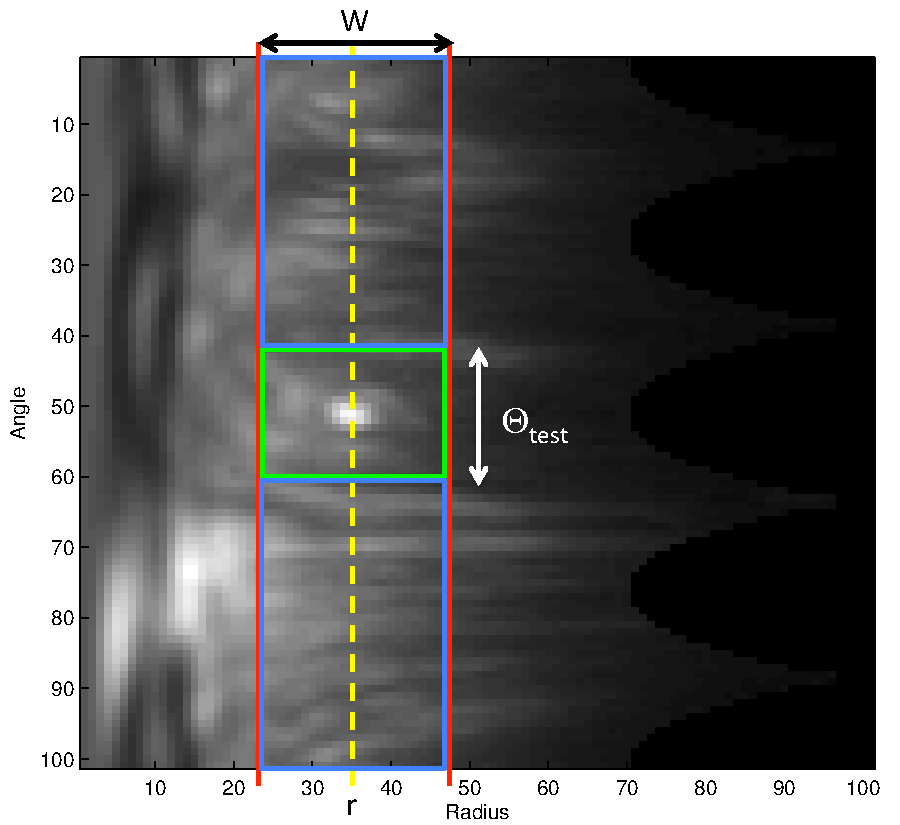
\includegraphics[width=4in]{figs/explain.pdf}
\end{center}
\vspace{-7mm}
\caption{}
\label{fig:spectrum}
\end{figure}
 

In the PCA step, we reformat the training set of patches into a
two-dimensional data matrix and find the singular value decomposition
(SVD).  This SVD returns the ranked list of principal components,
which are eigenvalue-ranked eigenvectors.  Each eigenvector can be
reformatted back into a $[W\times 3\times\Lambda\times 1]$ synthetic
patch; the model for the patches is arbitrary linear combinations of
the first $K$ eigenvectors from the PCA.  $K$ is a control parameter
controlling the freedom of the model.  As per usual, the PCA step
makes no use of any uncertainty estimates for the input data; the
first $K$ eigenvectors span the $K$-dimensional subspace of the full
data space that contains most of the variance of the original data.

Given the $K$ top eigenvectors from the training set, each patch in
the test set can be reconstructed by finding the linear combination
that minimizes the total squared reconstruction error (residual).
Again, at this reconstruction set, we do not use any uncertainty or
noise estimates for the data.  We perform this reconstruction for each
patch $P_{r \theta n}$ at a number of different values of $K$, saving
the patch residual $\Delta P^{(K)}_{r \theta n}$, which has the same
dimensions as the original patch but contains the residual data minus
reconstruction.

If there happens to be a companion centered at location $(r, \theta,
n)$ and if the model is not so free (for at least some values of $K$)
that it can fully absorb it, then (for at least some values of $K$)
the residuals $\Delta P^{(K)}_{r \theta n}$ ought to look something
like a companion.  In order to test this hypothesis, we
cross-correlate the residuals $\Delta P^{(K)}_{r \theta n}$ with a
patch-shaped \emph{rigid companion model}.  The cross-correlation
looks like a normalized dot product between the residuals and the
rigid companion model.  [we could use an equation here].  The rigid
companion model is, at each wavelength index $\lambda$, the $[W\times
  3\times 1\times 1]$ image of the point-spread function appropriate
for that wavelength in that exposure.  The model is rigid in the sense
that it has no free parameters.  In particular, the companion model
has a ``white spectrum'' in the sense that it has been given a
constant amplitude across wavelengths in the units of the original
calibrated data output from the instrument.  That's not realistic.
The amplitude of the cross-correlation with the rigid companion model
constitutes a detection signal, which can be seen as living in the
$(r, \theta ,n)$ space, or can be combined with other exposures to
live in a $(r, \theta)$ space, or can be transformed back to the
original imaging $(x, y)$ space.

\begin{figure}[h!]
\begin{center}
\mbox{
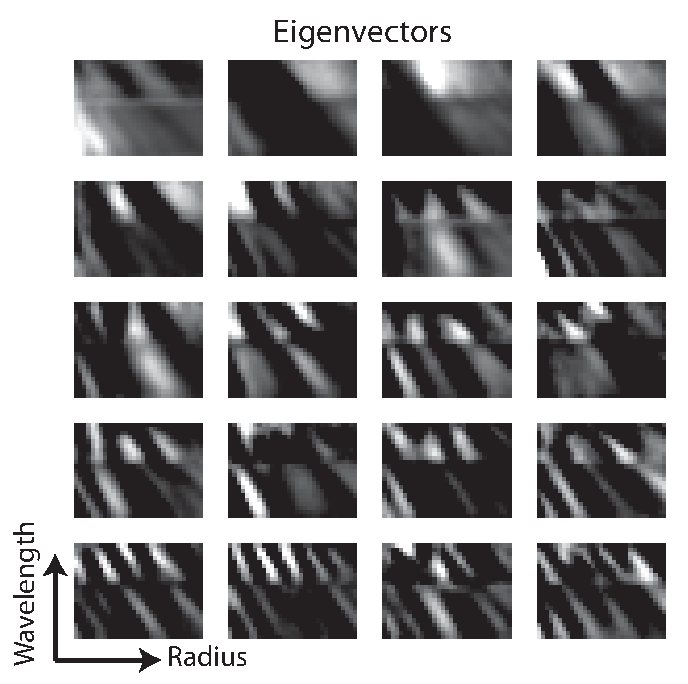
\includegraphics[width=2.5in]{figs/eigenvectors.pdf}
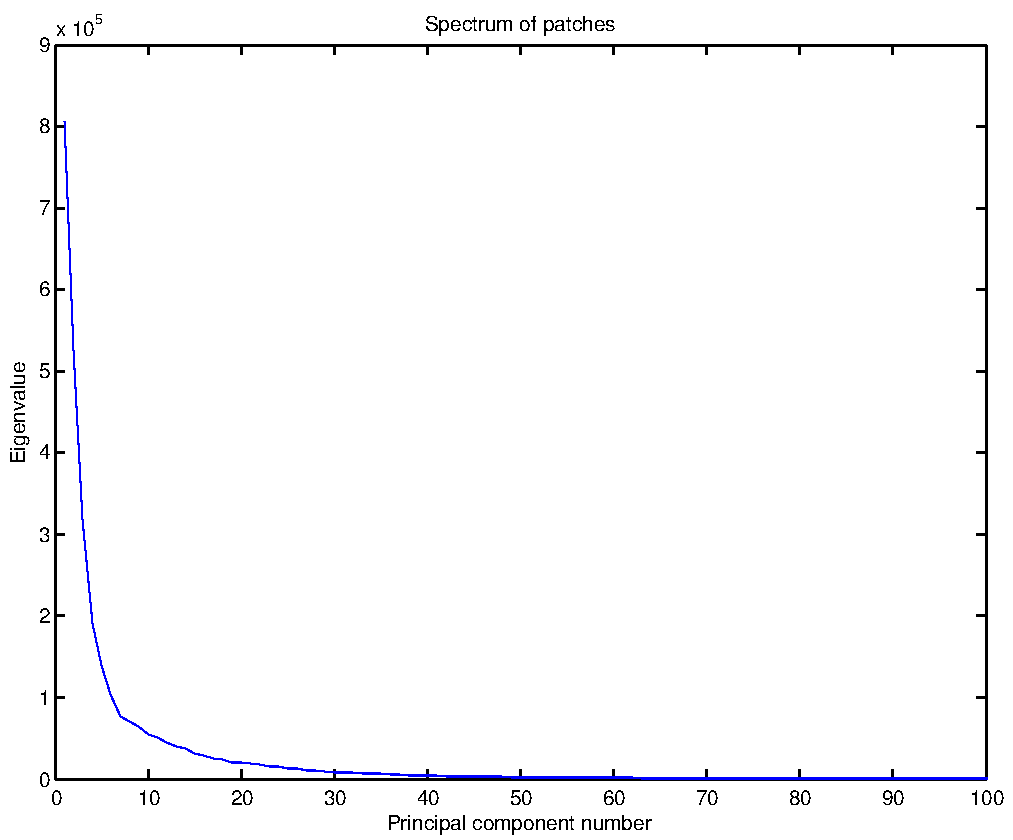
\includegraphics[width=3.1in]{figs/spectrum.pdf}
}
\end{center}
\vspace{-7mm}
\caption{}
\label{fig:spectrum}
\end{figure}
 
\begin{figure}[h!]
\begin{center}
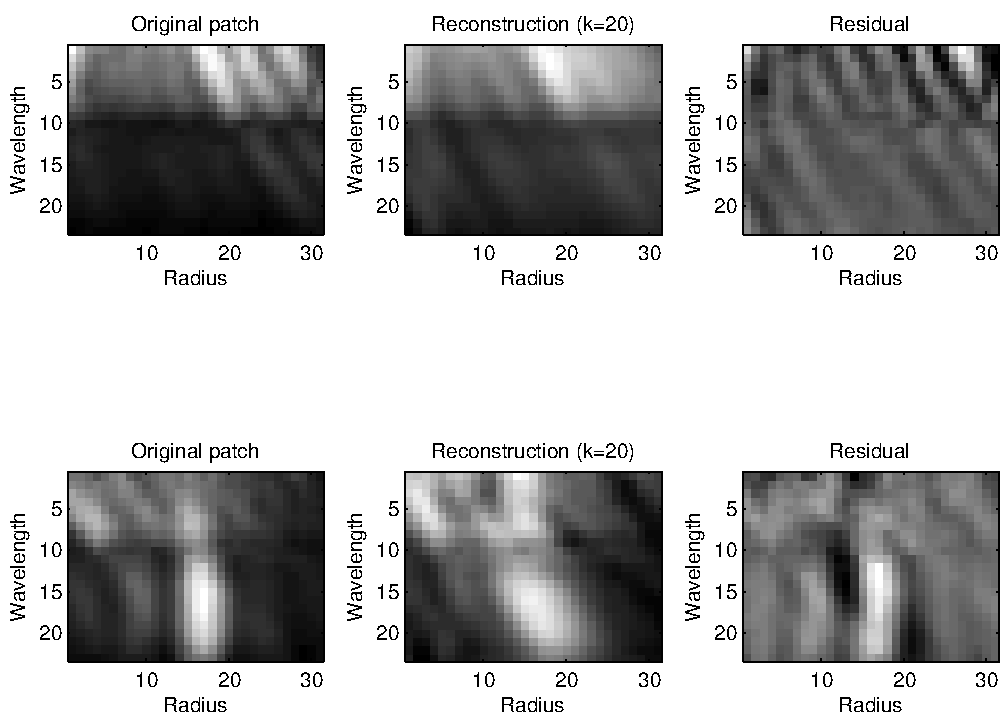
\includegraphics[width=5in]{figs/patch_reconstructions.pdf}
\end{center}
\vspace{-7mm}
\caption{}
\label{fig:patch_recon}
\end{figure}
  
 
...beat residuals against a flexible planet model for measurement...

...In summary, the method is...

\section{Results}

\begin{table}
\vspace{-15pt}
\begin{center}
\begin{tabular} { | c | c | c || c | c | c | c | c | c | c | c | } \hline
 Location & X & Y & 0.5\% &  1\% &  2\%  &  3\%  & 4 \% & 5\% & 7.5\%
 & 10\% \\ \hline \hline
 1    &   35  &    70  &   32  &    16  &    1  &     1  &     1  &     1   &    1  &     1\\ \hline
2    &   40  &    30  &  7  &    16  &    1  &     1  &     1  &     1   &    1  &     1\\ \hline
3    &   60  &    70  &   -  &    5  &    1  &     1  &     1  &     1   &    1  &     1\\ \hline
 4    &   65  &   35  &   27  &   21  &    3  &     1  &     1  &     1   &    1  &     1\\ \hline
\end{tabular}
\end{center}
\caption{Synthetic companion insertion on HD87696. Blob rank shown for 4 different locations.}
\label{table:result1}
\end{table}


\begin{figure}[h!]
\begin{center}
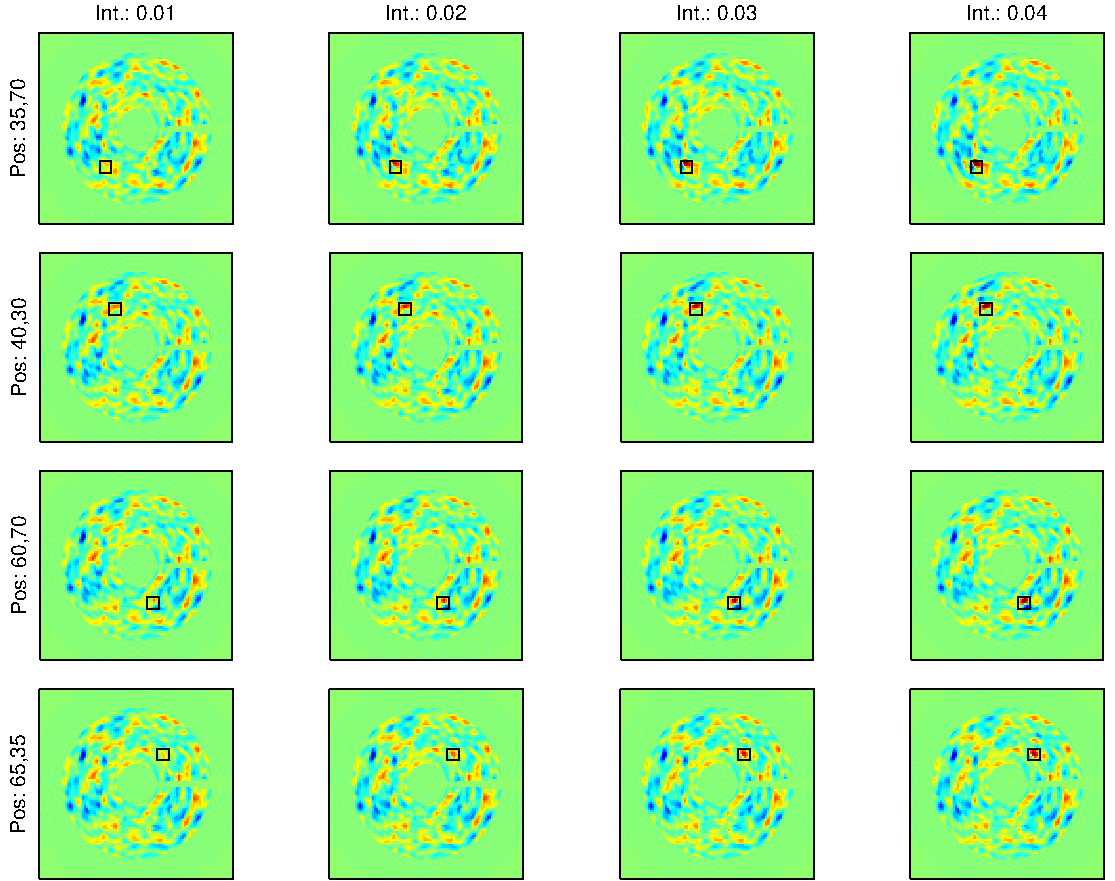
\includegraphics[width=5in]{figs/maps.pdf}
\end{center}
\vspace{-7mm}
\caption{}
\label{fig:results1}
\end{figure}

...Show results on, say, two stars, plus comparison to previous
outputs, maybe?...

\section{Discussion}

We have shown that a very flexible model for the unblocked light and a
model for a point-source companion can be used to make very precise
detections and measurements of faint companions in the high
dynamic-range spectroscopic imaging \project{P1640} instrument.  The
performance of our system is better by an order of magnitude than
existing methods for detecting faint companions.

There are a number of issues with the methods we have presented here;
work on these could further improve performance: We don't use a proper
instrument noise model in the construction of the model.  It would be
better to modify the PCA operation so that it makes use of the known
noise properties of the instrument (such as that of \citealt{hmf}).
In our mixture model (unblocked light plus planet), the planet model
is very rigid; it contains a particular SED assumption at the
detection step, and doesn't have enough angular flexibility to capture
possibly significant point-spread function morphology and variability.
Not surprisingly, the data-driven model we use is \emph{data starved};
it takes an enormous amount of data to fully constrain a flexible
data-driven model.  The model will get better as more data get taken
of a wider range of objects over a wider range of instrument and
atmsopheric conditions.  Related to this, the model we use does not
take as input any meta data about the telescope attitude (think
``gravitational loading'' and ``differential chromatic refraction'')
or observing conditions in training.  Data taken at different
altitudes show regularities that a more sophisticated model could
capture and use.  Another related limitation is that we treated the
data on different stars independently whereas data from multiple stars
could be combined for some aspects of model training.

...Why will similar effects exist in other existing and future
ground-based imagers?...Why will they exist in TPF and space-based
instruments?...What next?...

\acknowledgements It is a pleasure to thank [insert names here].  RF
was partially supported by [grant numbers here and same for DWH, BRO,
  DB etc].  Do we need an acknowledgement for \project{P1640}, Palomar
observers, and so on?

\begin{thebibliography}{}
\bibitem[Oppenheimer \etal(1875)]{p1640}
Oppenheimer,~B.~R. \etal, some P1640 publication
\bibitem[Tsalmantza \& Hogg(2012)]{hmf}
Tsalmantza,~P. \& Hogg,~D.~W., 2012, arXiv:1201.3370
\end{thebibliography}

\end{document}
